\documentclass{llncs}

\usepackage{graphicx}
\usepackage[hyphens]{url}
\usepackage{booktabs}
\usepackage{paralist}

% natbib for refs
%\usepackage[numbers,sort]{natbib} 

\begin{document}

\title{Popularity and Geospatial Spread of Trends on Twitter: A Middle
Eastern Case Study}

\author{Nabeel Albishry\inst{1,3}\thanks{This work has been supported by a doctoral research scholarship for
Nabeel Albishry from King Abdulaziz University, Kingdom of Saudi
Arabia.} \and Tom
  Crick\inst{2} \and Tesleem Fagade\inst{1} \and Theo Tryfonas\inst{1}}


\institute{Faculty of Engineering, University of Bristol, UK\\\email{\{n.albishry,tesleem.fagade,theo.tryfonas\}@bristol.ac.uk}
\and 
Department of Computer Science, Swansea University, UK\\\email{thomas.crick@swansea.ac.uk}
\and
Faculty of Computing \& IT, King Abdulaziz University, Jeddah, Saudi Arabia\\\email{nalbishry@kau.edu.sa}}
\maketitle

\begin{abstract}
Thousands of topics trend on Twitter across the world every day,
making it challenging to provide in-depth analysis of current issues,
topics and themes being discussed across various locations and
jurisdictions. There is thus a demand for simple and extensible
approaches to provide deeper insight into these trends and how they
propagate across locales. This paper represents one of the first
studies to look at geospatial spread of trends on Twitter, presenting
various techniques to provide increased understanding of how trends on
social networks can spread across various regions and nations. It is
based on a year-long data collection ({\emph{N}}=2,307,163) and
analysis between 2016-2017 of seven Middle Eastern countries (Bahrain,
Egypt, Kuwait, Lebanon, Qatar, Saudi Arabia, and the United Arab
Emirates). Using this year-long dataset, the project investigates the
popularity and geospatial spread of trends, focusing on trend
information but not processing individual topics, with the findings
showing that likelihood of trends spreading to other locales is to a
large extent influenced by the place in which it first appeared.
 \end{abstract}

\begin{keywords}
Trends, topic spread, popularity, network graphs, Twitter
\end{keywords}

\section{Introduction}\label{intro}

With the huge daily volume of generated content on Twitter -- c.500
million tweets per day -- trending topics serve as valuable sources of
information on highlighting what is going on in the world, or in
specific locations. Apart from the ``official'' trend lists provided
by the platform (on the website or through API endpoints), generating
insight from trends and topics detection has been receiving increasing
attention from across a variety of big social data-driven research
domains. In health for example, monitoring and analysis of trending
topics on social media has been adopted to measure emerging public
health issues, such as the spread of
influenza~\cite{Achrekar2011,Parker2013,Parker2015}. Furthermore,
across the marketing and business domains, topic detection and
classification are valuable approaches to extract knowledge and
insight on public opinions from posts on social
media~\cite{blamey-et-al-2012,Bello2013,albishry-et-al:ssei2018},
including analysing voting intentions and political view of
users~\cite{Fang2015}.

With the increasing popularity and use of social networks across a
wide range of domains, the impact of trends on public opinion and
perceptions has transformed social media campaigns and public
relations strategy. This has made trends a valuable target for
manipulation~\cite{Zhang2017}, stuffing~\cite{Irani2010},
spamming~\cite{Sedhai2015,Chu2012}, and
hijacking~\cite{VanDam2016}. Interestingly, deeper analysis of trend
hijacking cases suggests that increasing social media engagement may
not always be beneficial for public relations
strategies~\cite{Sanderson2016}.

A common approach in analysing Twitter trends is through clustering
and classification of trending topics based on
content~\cite{Zubiaga2011,Benhardus2013,Ferragina2015,albishry-et-al:iccci2017}.
The study in~\cite{TenThij2016} presented a content-independent method
to model trends progression through the dynamics of users
interactions; other studies have also attempted to provide real-time
classification or detection of
trends~\cite{Mathioudakis2010,Zubiaga2015}. With the increasing demand
for trends analysis across various domains, customisable clustering
tools that can be used by non-technical users have started to emerge,
such as the recent example introduced in~\cite{Arn2018}.


\section{Methodology}\label{method}

\subsection{Locales}

Seven Middle Eastern countries were selected for this study: Bahrain,
Egypt, Kuwait, Lebanon, Qatar, Saudi Arabia, and the United Arab
Emirates (UAE). The selection includes countries with relatively large
population (e.g. Egypt: 97,553,000) and relatively small populations
(e.g. Bahrain:
1,493,000)~\cite{UnitedNationsDepartmentofEconomicandSocialAffairs2017}.
Kuwait is reported to have the most active daily users on
Twitter~\cite{Salem2017}; as of March 2016, Saudi Arabia and Egypt
generated 33\% and 20\% of the tweets in the Middle Eastern
region. Bahrain is the most balanced location in terms of gender
breakdown of active users. Interestingly, between March 2014 and March
2016, Lebanon was the only location in the Middle Eastern states that
has not seen growth in active users, while UAE increased by 60\%. The
Gulf Cooperation Council countries -- Bahrain, Kuwait, Qatar, UAE, and
Saudi Arabia -- were reported to have the highest penetration
rates~\cite{Salem2017}.

\subsection{Data Collection}

Trending topic lists in the seven countries were monitored for a year
between October 2016 and October 2017. Every hour, trending lists were
collected through the Twitter REST API, which resulted in 7,948 hour's
worth of records for all the countries, totalling 2,307,163 trend
records. It is important to note that the Twitter API does not
necessarily provide trends data for every request; for example, it is
possible to receive no information for tweet volume. For each
location, the list of available trending topic is returned. From this
list, four pieces of information are extracted from each trend record:

\begin{itemize}
\item {\emph{woeid}}: the Yahoo! Where On Earth ID (WOEID) of the location;
\item {\emph{name}}: text of trending topic (e.g `{\texttt{\#Call\_For\_Action}}');
\item {\emph{as\_of}}: recorded timestamp of the trend;
\item {\emph{tweet\_volume}}: volume of tweets over the past 24 hours, if available.
\end{itemize}

While the Twitter API returns a list of trending topics for a specific
{\emph{woeid}} location, the tweet volumes do not provide a
comprehensive measure of the tweeting activity in that
location. Rather, the tweet volume refers to the overall number of
tweets containing the trend, regardless of their location. Although
the Twitter
documentation\footnote{\url{https://developer.twitter.com/en/docs/trends/trends-for-location/api-reference/get-trends-place}}
does not provide the necessary detail on this, it was apparent after
observing trends that showed up in various locations. Trends were
found with the same tweet volume across all locations and, hence,
participation volume of each location was not possible to be
accurately measured. Therefore, the context of this study does not
include any reference to this volume entity.

\subsection{Graph Construction}

The study is based on generating graph structures and conducting
analyses of their properties. The analysis approach involves
constructing two graphs; the {\emph{temporal base graph}} that
captures the structure of trend raw data, and the {\emph{weighted
aggregated graph}} which is generated from the base graph to further
explore its structure to provide additional
insights. Figure~\ref{fig:graphexamples} illustrates these graphs; the
nodes and direction orientation of edges are the same in both
graphs. Thus, nodes with zero indegree identify places, while trend
nodes feature zero outdegree.

\begin{figure}[!htb] \centering
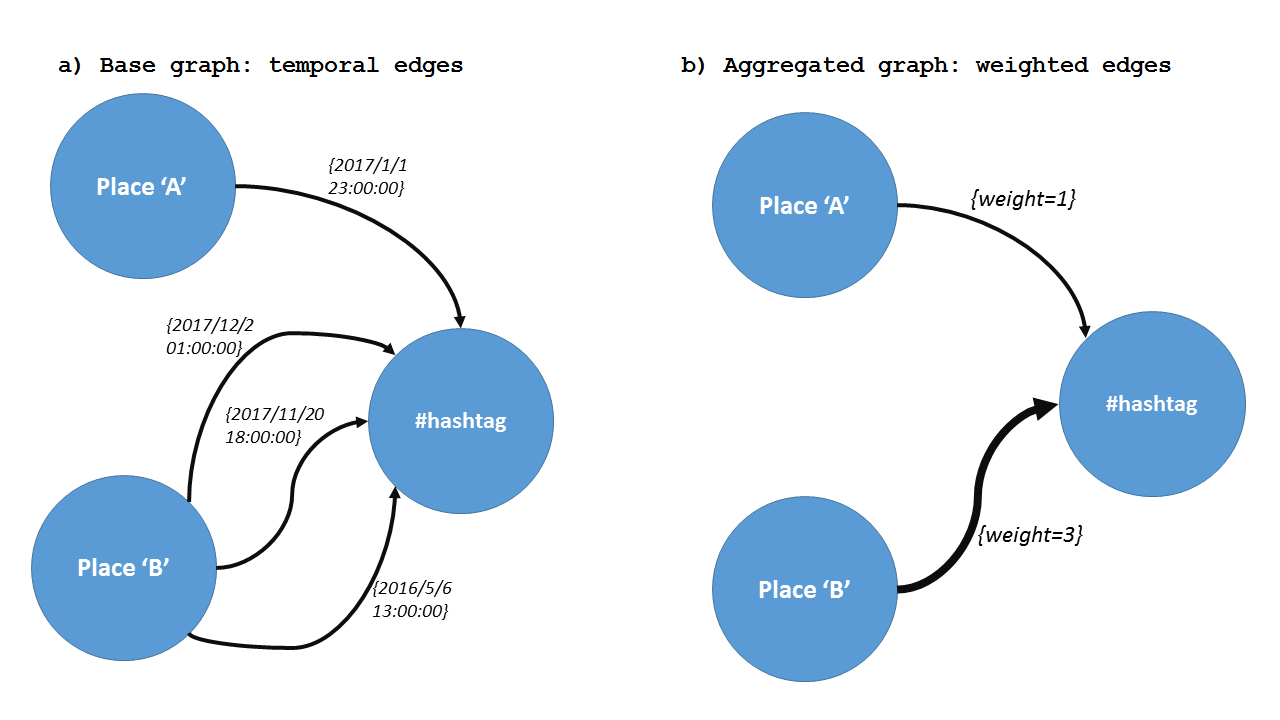
\includegraphics[width=\columnwidth]{images/graphexamples.png}
\caption{Graphs used in analyses}
\label{fig:graphexamples}
\end{figure}

The {\emph{temporal base graph}} is a directed graph that consists of
three trend entities: {\emph{place}}, {\emph{trend}} and
{\emph{timestamp}}. Nodes represent place and trends, and edges are
labelled with timestamps to indicate the time at which the trend
appeared in a location. This graph is used to examine temporal
properties, such as spread.

The {\emph{weighted aggregated graph}} is a graph that combines
temporal edges between two nodes (in the base graph) into a single
weighted edge. The feature of weighted edges in this graph is used to
measure the popularity of trends, repetition rate, participation of
countries, and the volume of the engagement.


\section{Results}\label{results}

Observation of the weighted graph provided an overall evaluation of
activity for trends and places. In total there were 76,266 distinct
trends that trended 2,307,163 times across all locations; this
suggests that trends may appear repeatedly over time. The overall
repetition ratio in the dataset was 97\%, and ranged from 80\% to 98\%
for individual locations, with Saudi Arabia scoring lowest and Qatar
scoring highest rate. {\emph{Indegree}}, {\emph{outdegree}}, and
{\emph{edges}} were used to conduct subsequent results, with further
explanation to follow in the relevant sections.

\subsection{Commonality and Popularity of Trends}

The node indegree indicates the number of locations at which the trend
showed ({\emph{commonality}}), and the weighted indegree is used to
measure the total number of times a trend showed
({\emph{popularity}}). Therefore, grouping trends based on indegree has
revealed 7 indegree groups, as shown in Table~\ref{tbl:trendsindegree}. 
Also, weighted indegree was used to analyse activity in these groups. 
Although 83\% of trends have appeared in one location only, their total 
weighted indegrees was 40\%; in other words, there were less common 
trends amongst locations, but their popularity was higher than isolated
trends\footnote{Isolated trends are those that have trended in one
place, i.e. their indegree equal 1.} -- this implies that trends
showing across multiple locations does not necessarily imply the prominance or
importance of activity or topic.

\begin{table}[!h]
\centering
\caption{Trends indegree groups}
\begin{tabular}{@{}crccccrr@{}}
\toprule
Indegree & No. trends & Ratio & Total W. & W. Ratio & Max. & Mean & Std \\ 
\midrule
1 & 62,959 & 0.826 & 936,959 & 0.406 & 2,146 &   14.88 &   43.26\\
2 &   7,338 & 0.096 & 335,073 & 0.145 & 1,957 &   45.66 &   77.45\\
3 &   2,840 & 0.037 & 220,805 & 0.096 & 1,842 &   77.75 &   96.29\\
4 &   1,538 & 0.020 & 216,524 & 0.094 & 2,797 & 140.78 & 201.03\\
5 &      850 & 0.011 & 184,127 & 0.080 & 3,604 & 216.62 & 297.36\\
6 &      463 & 0.006 & 192,968 & 0.084 & 3,998 & 416.78 & 581.76\\
7 &      278 & 0.004 & 220,707 & 0.096 & 5,367 & 793.91 & 994.66\\
\bottomrule
\end{tabular}
\label{tbl:trendsindegree}
\end{table}

\subsection{Location Participation}

The node outdegree reflects how many unique trends a location is
connected to ({\emph{diversity}}), and weighted outdegree measures the
ability of the location to generate trends ({\emph{activity}}). The
outdegree descriptive statistics, presented in
Table~\ref{tbl:locationoutdegree}, shows that Saudi Arabia came at the
top of the list, with 42\% of outgoing edges and weighing 20\% of the
total weight of the graph. Closeness in the table shows how close a
location node is to all other trend nodes; it shows that Saudi Arabia
has connections to 56\% of trends in the graph. Nevertheless, Saudi
Arabia was found lowest in terms of maximum edge weight, mean and
standard deviation; Qatar was found to have the reverse values. This
can be interpreted as the trends activity in Saudi Arabia was more
diverse in total, but more consistent. In contrast, Qatar is connected
to a limited number of trends with more focused activity. Also,
Qatar's outdegree is just 60\% of Bahrain's, although its weighted
degree was 1.9 higher.

\begin{table}[!h]
\centering
\caption{Location outdegree descriptive statistics}
\begin{tabular}{@{}lrccccccr@{}}
\toprule
Location & Outdegree & Out. ratio & W. Out. & W. Ratio & Closeness & Max. &  Mean & Std \\ 
\midrule
Bahrain &           7,424 & 0.07 & 133,069 & 0.06 & 0.10 & 1,949 & 17.92 &   78.48\\
Egypt &            14,282 & 0.14 & 383,830 & 0.17 & 0.19 & 1,408 & 26.88 &   58.68\\
Kuwait &          13,891 & 0.14 & 397,960 & 0.17 & 0.18 & 1,400 & 28.65 &   51.67\\
Lebanon &         6,044 & 0.06 & 294,761 & 0.13 & 0.08 & 2,146 & 48.77 & 133.64\\
Qatar &              4,484 & 0.04 & 248,003 & 0.11 & 0.06 & 2,173 & 55.31 & 146.79\\
Saudi Arabia & 42,767 & 0.42 & 468,081 & 0.20 & 0.56 & 1,175 & 10.95 &   17.43\\
UAE &              12,389 & 0.12 & 381,459 & 0.17 & 0.16 & 1,655 & 30.79 &   70.75\\
\bottomrule
\end{tabular}
\label{tbl:locationoutdegree}
\end{table}

\subsection{Edges Properties}

Edge weights in the graph were utilised to evaluate location activity
in indegree groups, as shown in
Figure~\ref{fig:indegreegrouptrends}. Overall, most of location
activity went to common trends. Although Saudi Arabia was the highest
in terms of total activity, the majority of its activity (61.26\%) was
identified as isolated trends. Moreover, observing originating
locations for isolated trends shows that 30\% of inbound edges came
from Saudi Arabia, as shown in
Figure~\ref{fig:weightedcontributions}. Egypt contributed the most in
2 and 3 indegree trend groups, UAE in 4, 5 and 6 indegree trends, and
for 7 indegree trends most of in edges originated from the Lebanon.

\begin{figure}[htb]
\centering
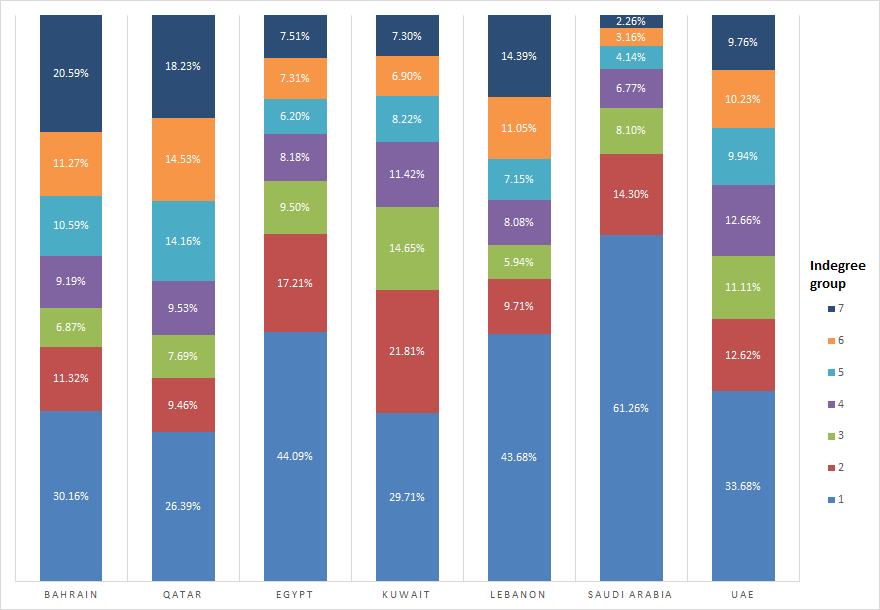
\includegraphics[width=\columnwidth]{images/indegreegrouptrends.png}
\caption{Trends Indegree group distributions across countries}
\label{fig:indegreegrouptrends}
\end{figure}

\begin{figure}[htb]
\centering
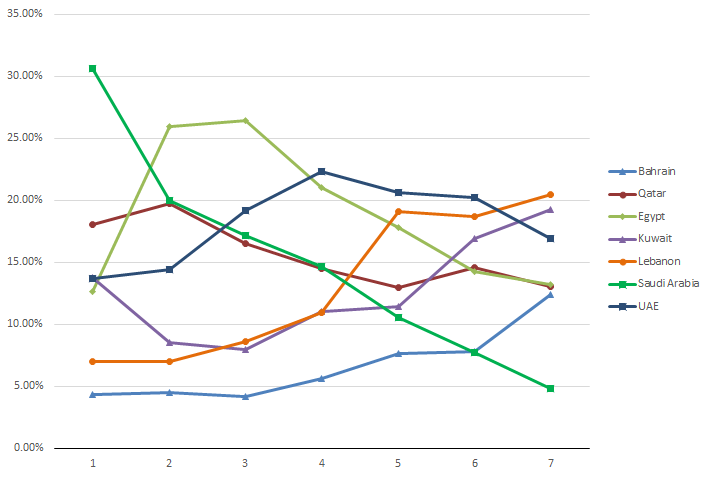
\includegraphics[width=\columnwidth]{images/weightedcontributions.png}
\caption{Weighted contribution of countries toward trends indegree groups}
\label{fig:weightedcontributions}
\end{figure}

\subsection{Temporal Spread and Reach}

As shown in Table~\ref{tbl:trendsindegree}, 60\% of weighted
indegree was associated with common trends. To further examine temporal
changes on those trends, timestamps on in-edges of trend nodes in the
temporal graph were observed. Those timestamps were used to measure
temporal order of locations for trend, as shown in
Table~\ref{tbl:temporders}. For instance, about 42\% of first
appearance of trends was in Saudi Arabia, while 36\% of 7th trend
appearance was in Bahrain.

\begin{table}[!h]
\centering
\caption{Distribution of temporal orders of location for multi-indegree trends}
\begin{tabular}{@{}lrrrrrrr@{}}
\toprule
Location & 1st & 2nd & 3rd & 4th & 5th & 6th & 7th \\ 
\midrule
Bahrain &          2.3 &    3.0 &    3.5 &  6.3 & 14.9 & 26.0 & 36.0 \\
Egypt &            16.3 & 13.2 & 21.3 & 22.8 & 16.8 & 11.7 &   2.5 \\
Kuwait &          16.5 & 29.5 & 23.8 & 15.1 & 13.2 & 11.2 &   8.3\\
Lebanon &         5.7 &   5.4 &   6.2 &   7.0 &   8.7 & 11.3 & 23.7 \\
Qatar &              4.1 &   4.9 &   8.9 & 16.1 & 25.1 & 25.6 & 12.6 \\
Saudi Arabia & 42.2 & 28.7 & 10.2 &   7.1 &   7.3 &   8.1 & 14.4 \\
UAE &              12.9 & 15.2 & 26.0 & 25.4 & 14.0 &   5.9 &   2.5\\
\midrule
{\emph{Total}} & 100 & 100 & 100 & 100 & 100 &  100 &   100\\
\bottomrule
\end{tabular}
\label{tbl:temporders}
\end{table}

A similar observation was made on the outdegree measures, with
timestamps on out-edges of place nodes in the temporal graph observed;
the results are presented in Table~\ref{tbl:appearanceorders}. The
highest portion of activities in Saudi Arabia, Egypt and Lebanon made
them 1st locations for trends to appear in. However, Bahrain, UAE, Qatar,
and Kuwait were more active with trends that have appeared previously.

\begin{table}[!h]
\centering
\caption{Distribution of appearance orders of locations}
\begin{tabular}{@{}lrrrrrrr@{}}
\toprule
Order & Bahrain & Saudi & Egypt & UAE & Lebanon & Qatar & Kuwait \\ 
\midrule
1st &  18.4 & 53.6 & 34.6 & 26.9 & 32.2 & 19.1 & 26.3 \\
2nd & 24.2 & 36.4 & 28.0 & 31.9 & 30.5 & 22.9 & 47.1\\
3rd &  12.8 & 5.8 & 20.3 & 24.4 & 15.8 & 18.6 &  17.1\\
4th &  12.1 & 2.1 & 11.4 & 12.5 & 9.3 & 17.6 & 5.7 \\
5th &  14.5 & 1.1 & 4.3 & 3.5 & 5.9 & 13.9 & 2.5 \\
6th &  11.8 & 0.6 & 1.4 & 0.7 & 3.6 &  6.6 & 1.0 \\
7th &  6.1 & 0.4 & 0.1 & 0.1 & 2.8 &  1.2 &  0.3\\
\midrule
{\emph{Total}} & 100 & 100 & 100 & 100 & 100 &  100 &   100\\
\bottomrule
\end{tabular}
\label{tbl:appearanceorders}
\end{table}

Additionally, the reach of trend was measured to examine how many
other locations a trend is likely to reach based on the location in which
it first appeared. Therefore, edges and related nodes relating to the
first column in Table~\ref{tbl:temporders} were used. The results
presented in Table~\ref{tbl:furtherreach} show that 62.3\% of trends
that first appeared in Kuwait have also appeared in exactly one more location,
and 5.1\% of those that first appeared in Qatar have also appeared in
six more locations.

\begin{table}[!h]
\centering
\caption{Further reach of trends per locations}
\begin{tabular}{@{}lrrrrrrr@{}}
\toprule
Reach & Bahrain & Egypt & UAE & Lebanon & Qatar & Kuwait & Saudi \\ 
\midrule
1 &  54.8 & 59.2 & 54.2 & 50.1 & 41.2 & 62.3 & 53.1 \\
2 &  19.3 & 22.7 & 21.2 & 21.3 & 24.3 & 18.9 & 21.7\\
3 &    8.3 & 9.8  & 11.1 & 10.4 & 12.6 & 10.1 & 13.2\\
4 &    8.3 & 4.4 & 6.4 & 8.1 & 12.0 & 4.1 & 7.2 \\
5 &    4.7 & 2.7 & 4.3 & 6.5 & 4.7 & 2.6 & 3.3 \\
6 &    4.7 & 1.2 & 2.8 & 3.7 & 5.1 & 2.1& 1.6\\
\midrule
{\emph{Total}} & 100 & 100 & 100 & 100 & 100 &  100 &   100\\
\bottomrule
\end{tabular}
\label{tbl:furtherreach}
\end{table}

Finally, Table~\ref{tbl:trendorigin} shows the origin of common trends
grouped by their indegree (connected places). As can be seen, 31.7\%
of trends that appeared in seven locations have originated from Saudi
Arabia, and 5\% from Bahrain. Nevertheless, Bahrain was better in
terms of further reach.

\begin{table}[!h]
\centering
\caption{Origin of trends per reached locations}
\begin{tabular}{@{}lrrrrrr@{}}
\toprule
Location & 2 & 3 & 4 & 5 & 6 & 7 \\ 
\midrule
Bahrain &           2.2 &   2.0 &   1.6 &   2.9 &   3.0 &    5.0 \\
Egypt &            17.5 & 17.3 & 13.8 & 11.3 & 12.5 &    9.4\\
Kuwait &          18.7 & 14.6  & 14.4 & 10.5 & 12.3 & 16.5\\
Lebanon &         5.2 &   5.7 &    5.1 &   7.2 & 10.6 & 10.1 \\
Qatar &              3.1 &   4.7 &    4.5 &   7.8 &   5.6 & 10.0 \\
Saudi Arabia & 40.7 & 42.9 &  48.1 & 47.4 & 40.2 & 31.7 \\
UAE &              12.7 & 12.8 &  12.4 & 12.9 & 15.8 & 17.3 \\
\midrule
{\emph{Total}} & 100 & 100 & 100 & 100 & 100 &  100 \\
\bottomrule
\end{tabular}
\label{tbl:trendorigin}
\end{table}

\vspace{-1em}
\section{Discussion and Conclusions}\label{dissconc}

From the results presented, we can see that isolated trends were found to be
most common across countries, although the study includes countries
with a high proportion of active users and high tweet generation rate,
such as Saudi Arabia and Egypt~\cite{Salem2017}. As previously
mentioned, the number of trends returned by the Twitter API does not
accurately reflect the true activity of the location. Low trending
topics may indicate low consensus on these discussed topics and does
not necessarily reflect tweeting activity. Also, the number of
trending topics is very likely to include repeated ones, and therefore
a high number of trends does not necessarily imply more new
topics. Furthermore, the number of trends was not found to correlate
with the tendency of location to participate in common trends. For
example, Saudi Arabia was found to be to connected to 56\% of trends,
however 61\% them were isolated trends i.e. trends that only appeared
in Saudi Arabia. Meanwhile, most of Qatar's trends (73.6\%) were
common ones, although it had edges with 6\% of trends; this indicates
that the activity of certain location is more focused on internal
issues and concerns.

Also, the further reach of trends (i.e. appearing in other locations)
was observed for each location. Although a specific location may do
well in reaching other locations, the number of trends it generates may
affect the total reach. For example, Qatar was highest in reaching
other locations, however it was the 5th in being the origin of trends
that reach all locations. This was certainly clear in the case of Saudi
Arabia: its scores in reaching other locations were not comparable to its
scores in being the origin of common trends, as shown in
Tables~\ref{tbl:furtherreach} and \ref{tbl:trendorigin}.

This study has presented an approach to analysing trends
data using graphs and their properties. It demonstrates the importance
of graph construction techniques to capture raw trends data, resulting
in the temporal base graph. Then, it presented how aggregated weighted
graph can be generated from the base graph. The temporal graph was
used to measure temporal properties such as spread and reach; the
weighted graph was used to measures overall activities, such as
commonality and popularity of trends, and diversity and activity of
locations.

The presented approach showed how trends data can be used to evaluate
topics and location activity without the need to crawl individual
topics. Also, it shows how to measure spread of trends and reach based
on their historical records as well as the originating location. This
approach can be used and extended to identify trends of important
features; for example, to extract high spread trends, or how likely it
is for a trend to reach a specific location from another one.


% \begin{acks}
% This work has been supported by a doctoral research scholarship for
% Nabeel Albishry from King Abdulaziz University, Kingdom of Saudi
% Arabia.
% \end{acks}


% bib
\bibliographystyle{splncs}
\bibliography{iccci2018}

\end{document}
